\documentclass{beamer}
\usepackage[utf8]{inputenc}
\usepackage[T1]{fontenc}
\usepackage[ngerman]{babel}
\usepackage{times}
\usepackage{graphicx}

\usetheme{Boadilla}

\title[EPM]{EPM\\Elastic Persistent Memory}

\author{Florian Klein}

\institute[Universität Düsseldorf] {Institut für Informatik\\Abteilung Betriebssysteme\\Heinrich-Heine-Universität Düsseldorf}

\date{12.06.2012}

\titlegraphic{
\includegraphics[width=3cm]{../img/hhulogo}}

\begin{document}

\section*{Titelfolie}

	\begin{frame}
		\titlepage
	\end{frame}

\section*{Gliederung}

	\begin{frame}
		\frametitle{Gliederung}

		\tableofcontents[hideallsubsections]
	\end{frame}

\section{Einführung}

	\begin{frame}
		\frametitle{Zielsetzung und Eigenschaften}

		\begin{block}{Zielsetzung}
			\begin{itemize}
				\item Alle Daten permanent im RAM
				\item Gute Fehlertoleranz (Knotenausfälle, Netzwerkpartitionierung, etc.)
				\item Skalierbar (mehrere tausend Knoten)
			\end{itemize}
		\end{block}

		\begin{block}{Eigenschaften}
			\begin{itemize}
				\item variable Konsistenz
				\item verteilte MetaDaten-Verwaltung
				\item Logging und FastRecovery
				\item konfigurierbar bzgl. des CAP-Dilemma
			\end{itemize}
		\end{block}
	\end{frame}

	\begin{frame}
		\frametitle{Einsatzmöglichkeiten und Anwendungsbeispiele}

		\begin{block}{Einsatzmöglichkeiten}
			\begin{itemize}
				\item Rechenzentren
				\item Cloud-Computing
				\item große Anwendungen mit hohem Datendurchsatz
			\end{itemize}
		\end{block}

		\begin{block}{Anwendungsbeispiele}
			\begin{itemize}
				\item verteiltes Dateisystem über Fuse-Anbindung
				\item Tabellenverwaltung (ähnlich zu BigTable)
					\begin{itemize}
						\item ACID-Kriterien über mehrere Zeilen
					\end{itemize}
				\item Cache
					\begin{itemize}
						\item Unterstützung von Timeouts und Read-Only-Einträgen
					\end{itemize}
				\item Data-Store
			\end{itemize}
		\end{block}
	\end{frame}

\section{Funktionen}

	\begin{frame}
		\frametitle{Gliederung}

		\tableofcontents[currentsection, hideothersubsections]
	\end{frame}

	\begin{frame}
		\frametitle{Konsistenz und Replikation}

		\begin{block}{unterstützte Konsistenzmodelle}
			\begin{itemize}
				\item schwache Konsistenz
				\item starke Konsistenz
				\item ggf. transaktionale Konsistenz
			\end{itemize}
		\end{block}

		\begin{block}{Replikation}
			\begin{itemize}
				\item feste oder dynamische Replikatanzahl
				\item Unterstützung von Erasure-Codes
				\item CAP-Dilema-Eigenschaften konfigurierbar
			\end{itemize}
		\end{block}
	\end{frame}

	\begin{frame}
		\frametitle{Fehlertoleranz und MetaDaten-Verwaltung}

		\begin{block}{Fehlertoleranz}
			\begin{itemize}
				\item Maskieren von Knotenausfälle
				\item Maskieren von Netzwerkpartitionen
				\item Verschmelzung von Netzwerkpartitionen
				\item lokales und entferntes Logging
				\item FastRecovery
			\end{itemize}
		\end{block}

		\begin{block}{MetaDaten-Verwaltung}
			\begin{itemize}
				\item verteilt in Form einer DHT
				\item lokaler Cache
			\end{itemize}
		\end{block}
	\end{frame}

	\begin{frame}
		\frametitle{Daten-Verwaltung}

		\begin{block}{Daten-Verwaltung}
			\begin{itemize}
				\item in Form von Binärblöcken variabler Größe (max. 100 MB)
				\item Jeder Binärblock hat eine eindeutige ID (512 Bit)
				\item Event-Service (Update / Invalidate)
				\item PubSub-Service
			\end{itemize}
		\end{block}

		\begin{block}{Schnittstelle}
			\begin{itemize}
				\item[] 
				\begin{enumerate}
					\item[create] erzeugt einen neuen Datenblock mit einer unbenutzen ID
					\item[get] Holt einen Datenblock (synchron oder asynchron))
					\item[put] Speichert bzw. Aktualisiert einen Datenblock
					\item[lock] Sperre auf einen Datenblock setzen (freiwillig oder advisory)
					\item[remove] löscht einen Datenblock
				\end{enumerate}
			\end{itemize}
		\end{block}
	\end{frame}

\section{Aufbau}

	\begin{frame}
		\frametitle{Gliederung}

		\tableofcontents[currentsection, hideothersubsections]
	\end{frame}

	\begin{frame}
		\frametitle{Aufbau}

		\begin{block}{Kern}
			\begin{itemize}
				\item Verwaltung der Datenblöcke und MetaDaten
				\item Datenmigration
				\item PubSub- und Event-Service
				\item Logging und FastRecovery
				\item Netzwerkkommunikation
			\end{itemize}
		\end{block}

		\begin{block}{Erweiterungen}
			\begin{itemize}
				\item Replikation und Konsistenzmodelle
				\item Namensdienst
				\item Tabellenverwaltung
				\item Fuse-Anbindung
			\end{itemize}
		\end{block}
	\end{frame}

	\begin{frame}
		\frametitle{Aufbau}

		\begin{block}{Überblick}
			\center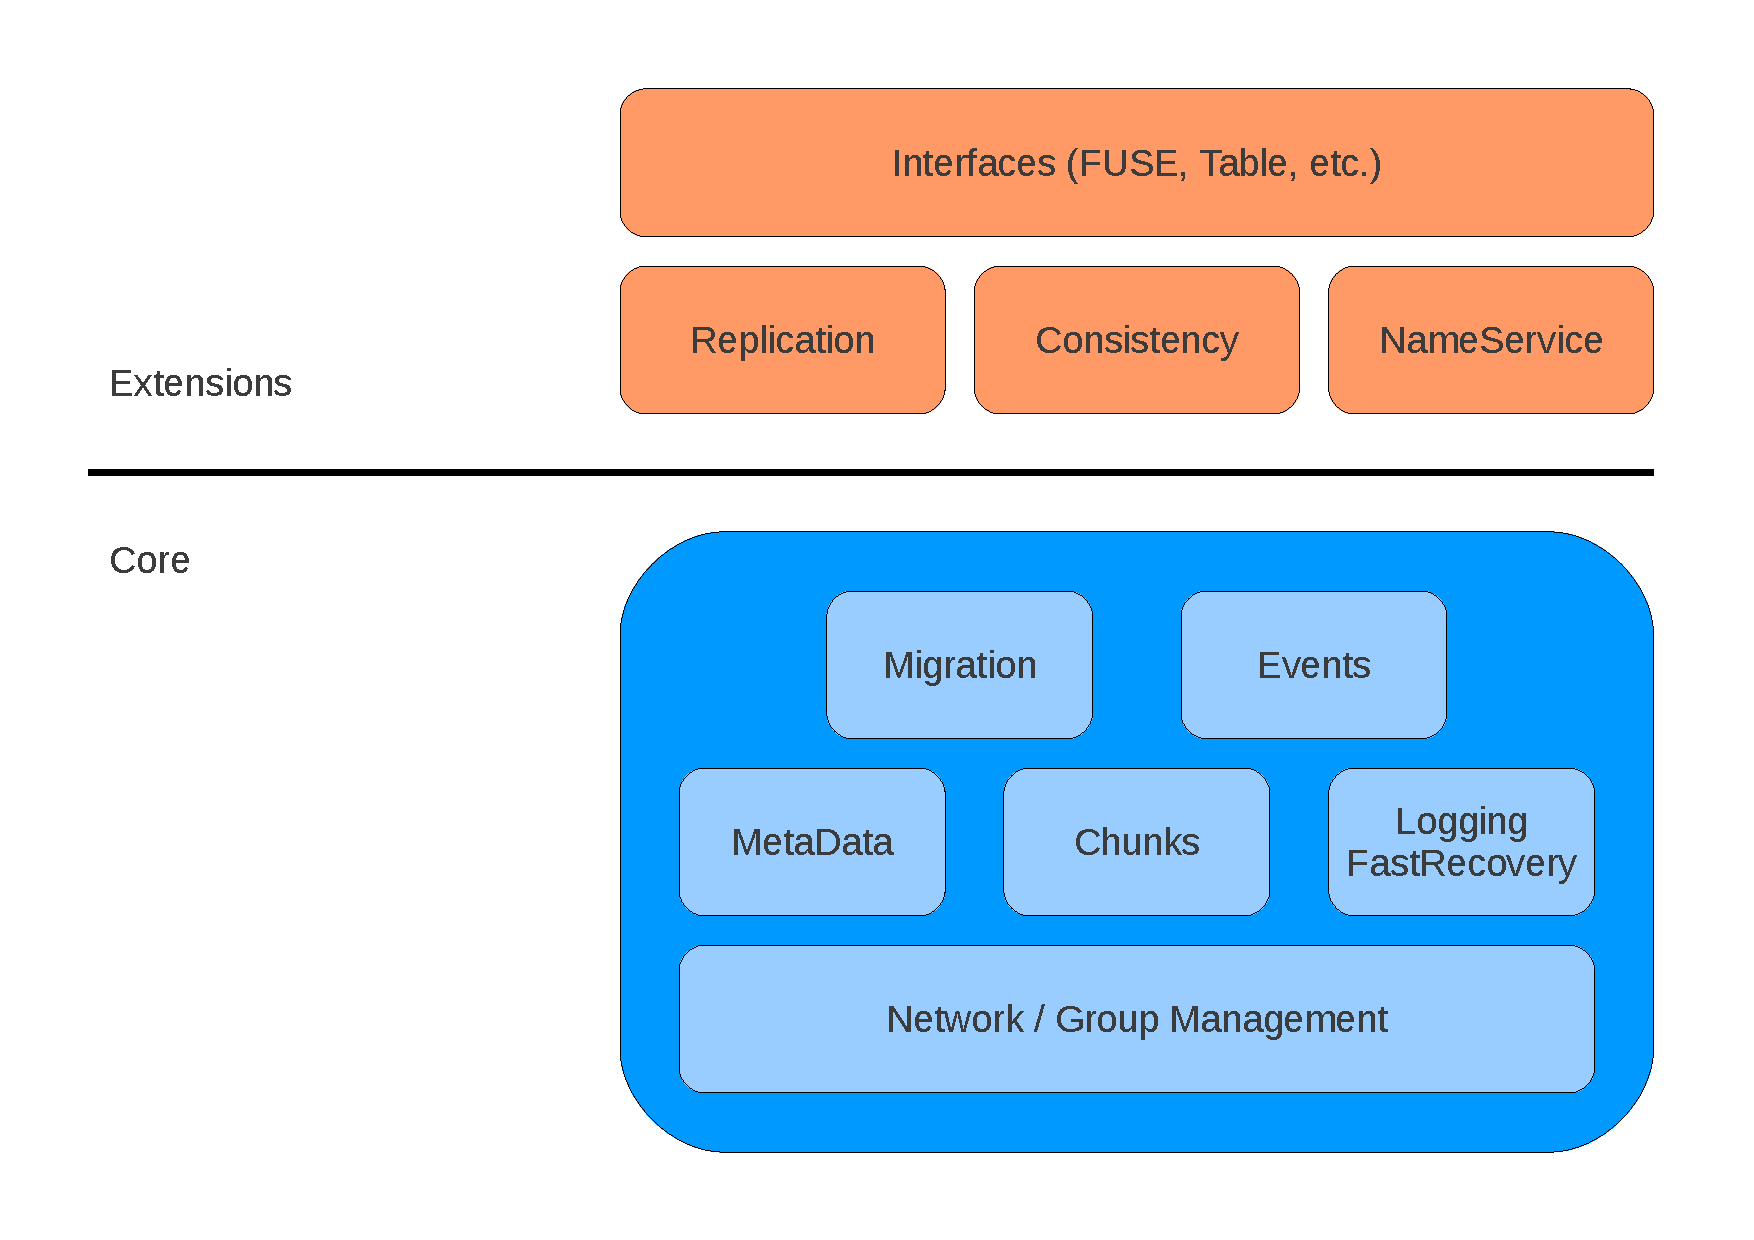
\includegraphics[width=9cm]{../img/aufbau}
		\end{block}
	\end{frame}

\section{Komponenten}

	\begin{frame}
		\frametitle{Gliederung}

		\tableofcontents[currentsection, hideothersubsections]
	\end{frame}

	\subsection{Datenblock-Verwaltung}

		\begin{frame}
			\frametitle{Datenblock-Verwaltung}

			\begin{block}{Struktur eines Datenblocks}
				\begin{itemize}
					\item Eindeutige 512-Bit ID
					\item Binärdaten in Form eines byte-Arrays
				\end{itemize}
			\end{block}

			\begin{block}{Eigenschaften}
				\begin{itemize}
					\item variable Größe der Datenblöcke (konfigurierbare maximal Größe)
					\item Eindeutige ID wird über einen Hash-Algorithmus erzeugt
					\item Synchrone und asynchrone Lesezugriffe
					\item Streaming API um unnötige Wartezeiten zu umgehen
					\item Lock-Mechanismus (freiwillige Sperre oder Advisory-Lock)
				\end{itemize}
			\end{block}
		\end{frame}

		\begin{frame}
			\frametitle{Datenblock-Verwaltung}
			\framesubtitle{Implementierung I}

			\begin{block}{create - Erzeugt eine neue BlockID}
				\begin{itemize}
					\item konfigurierbarer Hash-Algorithmus (default: SHA-512)
					\item Basis ist die lokale IP-Adresse und die aktuelle Zeit in Nanosekunden
				\end{itemize}
			\end{block}

			\begin{block}{get - Holt einen Datenblock anhand einer BlockID}
				\begin{enumerate}
					\item Prüfe den lokalen Speicher
						\begin{enumerate}
							\item[a)] Datenblock vorhanden $\rightarrow$ Bei Schritt 5 fortfahren
							\item[b)] Datenblock nicht vorhanden $\rightarrow$ Bei Schritt 2 fortfahren
						\end{enumerate}
					\item Über die MetaDaten-Verwaltung den Ziel-Rechner finden
					\item Anfrage an Ziel-Rechner stellen
					\item Antwort des Ziel-Rechners abwarten $\rightarrow$ Datenblock entgegen nehmen
					\item Datenblock zurückgeben
				\end{enumerate}
			\end{block}
		\end{frame}

		\begin{frame}
			\frametitle{Datenblock-Verwaltung}
			\framesubtitle{Implementierung II}

			\begin{block}{put - Speichert einen Datenblock}
				\begin{enumerate}
					\item Prüfe den lokalen Speicher
						\begin{enumerate}
							\item[a)] Datenblock vorhanden $\rightarrow$ Datenblock ersetzen
							\item[b)] Datenblock nicht vorhanden $\rightarrow$ Bei Schritt 2 fortfahren
						\end{enumerate}
					\item Über die MetaDaten-Verwaltung den Ziel-Rechner finden
						\begin{enumerate}
							\item[a)] lokale Rechner $\rightarrow$ Datenblock speichern (neuer Datenblock)
							\item[b)] anderer Rechner $\rightarrow$ Nachricht mit dem Datenblock an den Ziel-Rechner schicken
						\end{enumerate}
				\end{enumerate}
			\end{block}

			\begin{block}{remove - Löscht einen Datenblock}
				\begin{enumerate}
					\item Prüfe den lokalen Speicher
						\begin{enumerate}
							\item[a)] Datenblock vorhanden $\rightarrow$ Datenblock löschen
							\item[b)] Datenblock nicht vorhanden $\rightarrow$ Bei Schritt 2 fortfahren
						\end{enumerate}
					\item Über die MetaDaten-Verwaltung den Ziel-Rechner finden
					\item Nachricht an den Ziel-Rechner schicken
				\end{enumerate}
			\end{block}
		\end{frame}

		\begin{frame}
			\frametitle{Datenblock-Verwaltung}
			\framesubtitle{Implementierung III}

			\begin{block}{lock - Sperrt einen Datenblock}
				\begin{enumerate}
					\item Prüfe den lokalen Speicher
						\begin{enumerate}
							\item[a)] Datenblock vorhanden $\rightarrow$ Datenblock sperren und bei Schritt 5 fortfahren
							\item[b)] Datenblock nicht vorhanden $\rightarrow$ Bei Schritt 2 fortfahren
						\end{enumerate}
					\item Über die MetaDaten-Verwaltung den Ziel-Rechner finden
					\item Anfrage an Ziel-Rechner stellen
					\item Antwort des Ziel-Rechners abwarten $\rightarrow$ Datenblock entgegen nehmen
					\item Datenblock zurückgeben
				\end{enumerate}

				Die Sperre wird freigegeben, sobald der Datenblock mit \texttt{put} gespeichert wird.
			\end{block}
		\end{frame}

	\subsection{MetaDaten-Verwaltung}

		\begin{frame}
			\frametitle{MetaDaten-Verwaltung}

			\begin{block}{Aktueller Stand}
				\begin{itemize}
					\item ZooKeeper als zentrale Instanz
					\item ObjektID wird auf IP + Port des Zielrechners gemapped
					\item Verteilter Lock-Mechanismus
				\end{itemize}
			\end{block}

			\begin{block}{Aussicht}
				\begin{itemize}
					\item Verteilte Verwaltung mit Hilfe einer DHT
					\item lokaler Cache für Anfragen
				\end{itemize}
			\end{block}
		\end{frame}

	\subsection{Migration}

		\begin{frame}
			\frametitle{Migration}

			\begin{block}{Aktueller Stand}
				\begin{itemize}
					\item in die Datenblock-Verwaltung eingebunden
					\item Ablauf:
						\begin{enumerate}
							\item Datenblock an den Ziel-Rechner übertragen
							\item MetaDaten-Verwaltung benachrichtigen
							\item lokalen Datenblock löschen
							\item PubSub-Service wird aktuell nicht informiert
						\end{enumerate}
				\end{itemize}
			\end{block}

			\begin{block}{Aussicht}
				\begin{itemize}
					\item Eigenständige Komponente
					\item Datenblock während der Migration sperren
					\item automatische Lastverteilung durch Migrations-Algorithmus
					\item AKtualisierung des PubSub-Service
				\end{itemize}
			\end{block}
		\end{frame}

	\subsection{PubSub- und Event-Service}

		\begin{frame}
			\frametitle{PubSub- und Event-Service}

			\begin{block}{Aktueller Stand}
				\begin{itemize}
					\item in die Datenblock-Verwaltung eingebunden
					\item mögliche Subscribearten: Update, Invalidate
					\item lokale Verwaltung für jeden gespeicherten Datenblock
					\item Bei einer Aktualisierung wird zu jedem der Subscriber eine Verbindung aufgebaut und eine Nachricht verschickt
				\end{itemize}
			\end{block}

			\begin{block}{Aussicht}
				\begin{itemize}
					\item Eigenständige Komponente
					\item Gruppenkommunikation (beispielsweise jgroups)
					\item verteilte Verwaltung
					\item evtl. sogar aus dem Kern raus verlagern
				\end{itemize}
			\end{block}
		\end{frame}

	\subsection{Logging}

		\begin{frame}
			\frametitle{Logging}

			\begin{block}{Eigenschaften}
				\begin{itemize}
					\item Lokales Log
					\item Zusätzliche Backup-Logs auf weiteren Rechnern (default 3)
					\item Restart von lokalem Log möglich
					\item Log ist unterteilt in Segmente
						\begin{itemize}
							\item Segmente sind wiederum unterteilt in Blöcke
							\item Verwaltung der Segmente erfolgt mit Hilfe iner Hash-Tabelle
						\end{itemize}
					\item zusätzlich zu den Datenblöcken wird eine Versionsnummer pro Datenblock gepflegt
				\end{itemize}
			\end{block}
		\end{frame}

		\begin{frame}
			\frametitle{Logging}

			\begin{block}{Struktur}
				\center\includegraphics[width=9cm]{../img/logging_struktur}
			\end{block}
		\end{frame}

		\begin{frame}
			\frametitle{Logging}
			\framesubtitle{Funktionsweise I}

			\begin{block}{Neuen Datenblock speichern}
				\begin{enumerate}
					\item Finde eine Anzahl von zusammenhängenden Blöcken mit der Größe $\geq$ Größe des Datenblocks
						\begin{itemize}
							\item Ist dies nicht möglich, wird ein neues Segment erstellt
						\end{itemize}
					\item Speicher den Datenblock in den ausgewählten Blöcken (Versionsnummer = 1)
					\item Aktualisiere den Segement-Header
					\item Aktualisiere die Hash-Tabelle mit den MetaDaten
				\end{enumerate}
			\end{block}

			\begin{block}{Datenblock löschen}
				\begin{enumerate}
					\item Lösche die entsprechenden Einträge im Segment-Header für jeden belegten Block
					\item Aktualisiere die Hash-Tabelle mit den MetaDaten
				\end{enumerate}
			\end{block}
		\end{frame}

		\begin{frame}
			\frametitle{Logging}
			\framesubtitle{Funktionsweise II}

			\begin{block}{Datenblock ändern}
				\begin{enumerate}
					\item Vergleiche die Größe des gespeicherten Datenblocks mit der neuen Größe
						\begin{enumerate}
							\item[a)] die Größe ist gleich $\rightarrow$ die Blöcke mit den neuen Daten überschreiben
							\item[b)] die Größe hat sich verringert $\rightarrow$ die Blöcke mit den neuen Daten überschreiben und ggf. leere Blöcke freigeben
							\item[c)] die Größe hat sich erhöht $\rightarrow$ benachbarte Böcken überprüfen
								\begin{enumerate}
									\item[a)] Genügend freie Blöcke vorhanden $\rightarrow$ die Daten in den Blöcken speichern
									\item[b)] Nicht genügend freie Blöck vorhanden $\rightarrow$ Die bisher belegten Blöcke freigeben und einen neuen Speicherplatz suchen (siehe neuen Datenblock speichern)
								\end{enumerate}
						\end{enumerate}
					\item Versionsnummer inkrementieren
					\item Aktualisiere den Segement-Header
					\item Aktualisiere die Hash-Tabelle mit den MetaDaten
				\end{enumerate}
			\end{block}
		\end{frame}

	\subsection{FastRecovery}

		\begin{frame}
			\frametitle{FastRecovery}

			\begin{block}{Ablauf}
				\begin{enumerate}
					\item ein Knoten fällt aus
					\item einer der Backup-Knoten bemerkt den Ausfall und benachrichtigt die anderen Backup-Knoten
					\item die Backup-Knoten initialisieren den Recovery-Algorithmus (Init-Phase)
					\item die Backup-Knoten teilen die wiederherzustellenden Datenblöcke untereinander auf (Divide-Phase)
					\item die Datenblöcke werden lokal wiederhergestellt (Recover-Phase)
				\end{enumerate}
			\end{block}
		\end{frame}

		\begin{frame}
			\frametitle{FastRecovery}

			\begin{block}{Init-Phase}
				\center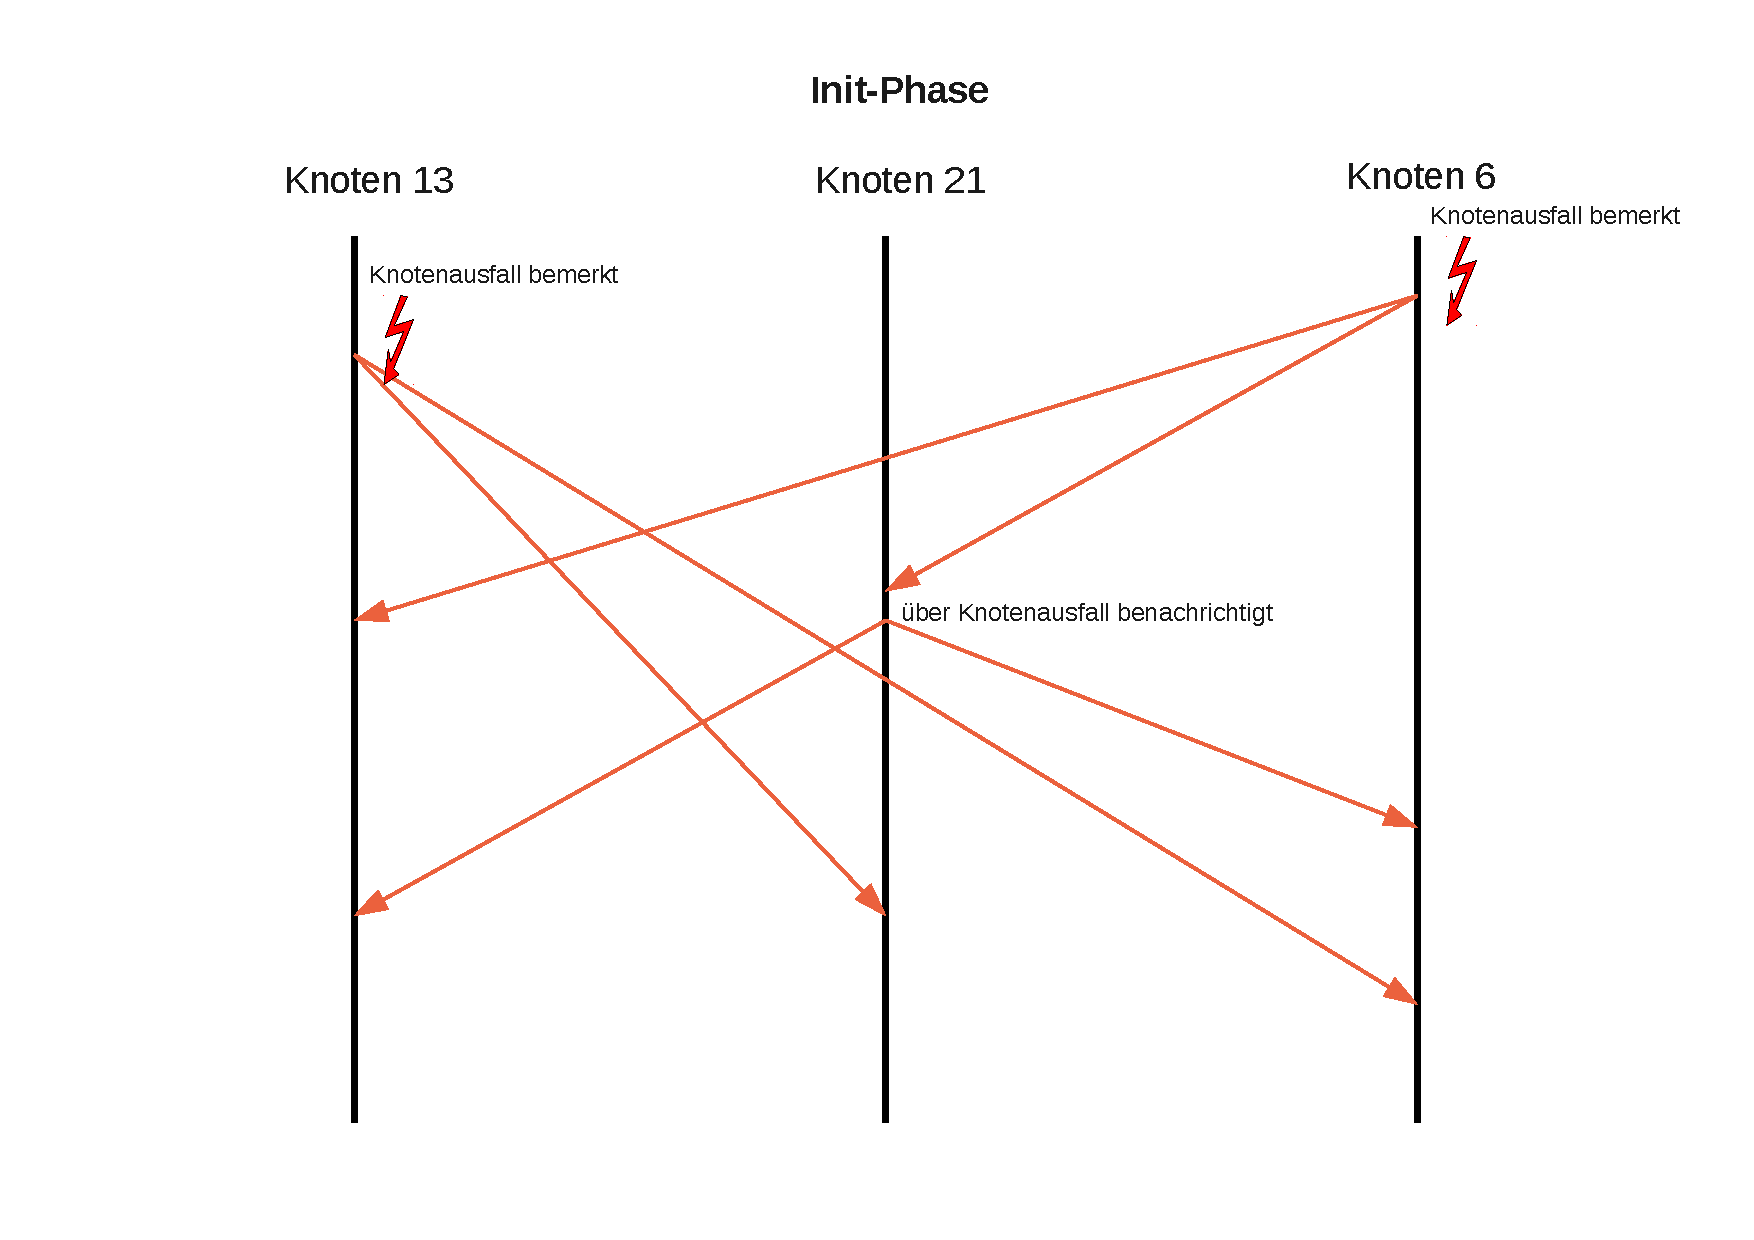
\includegraphics[width=9cm]{../img/recovery_init}
			\end{block}
		\end{frame}

		\begin{frame}
			\frametitle{FastRecovery}

			\begin{block}{Divide-Phase}
				\center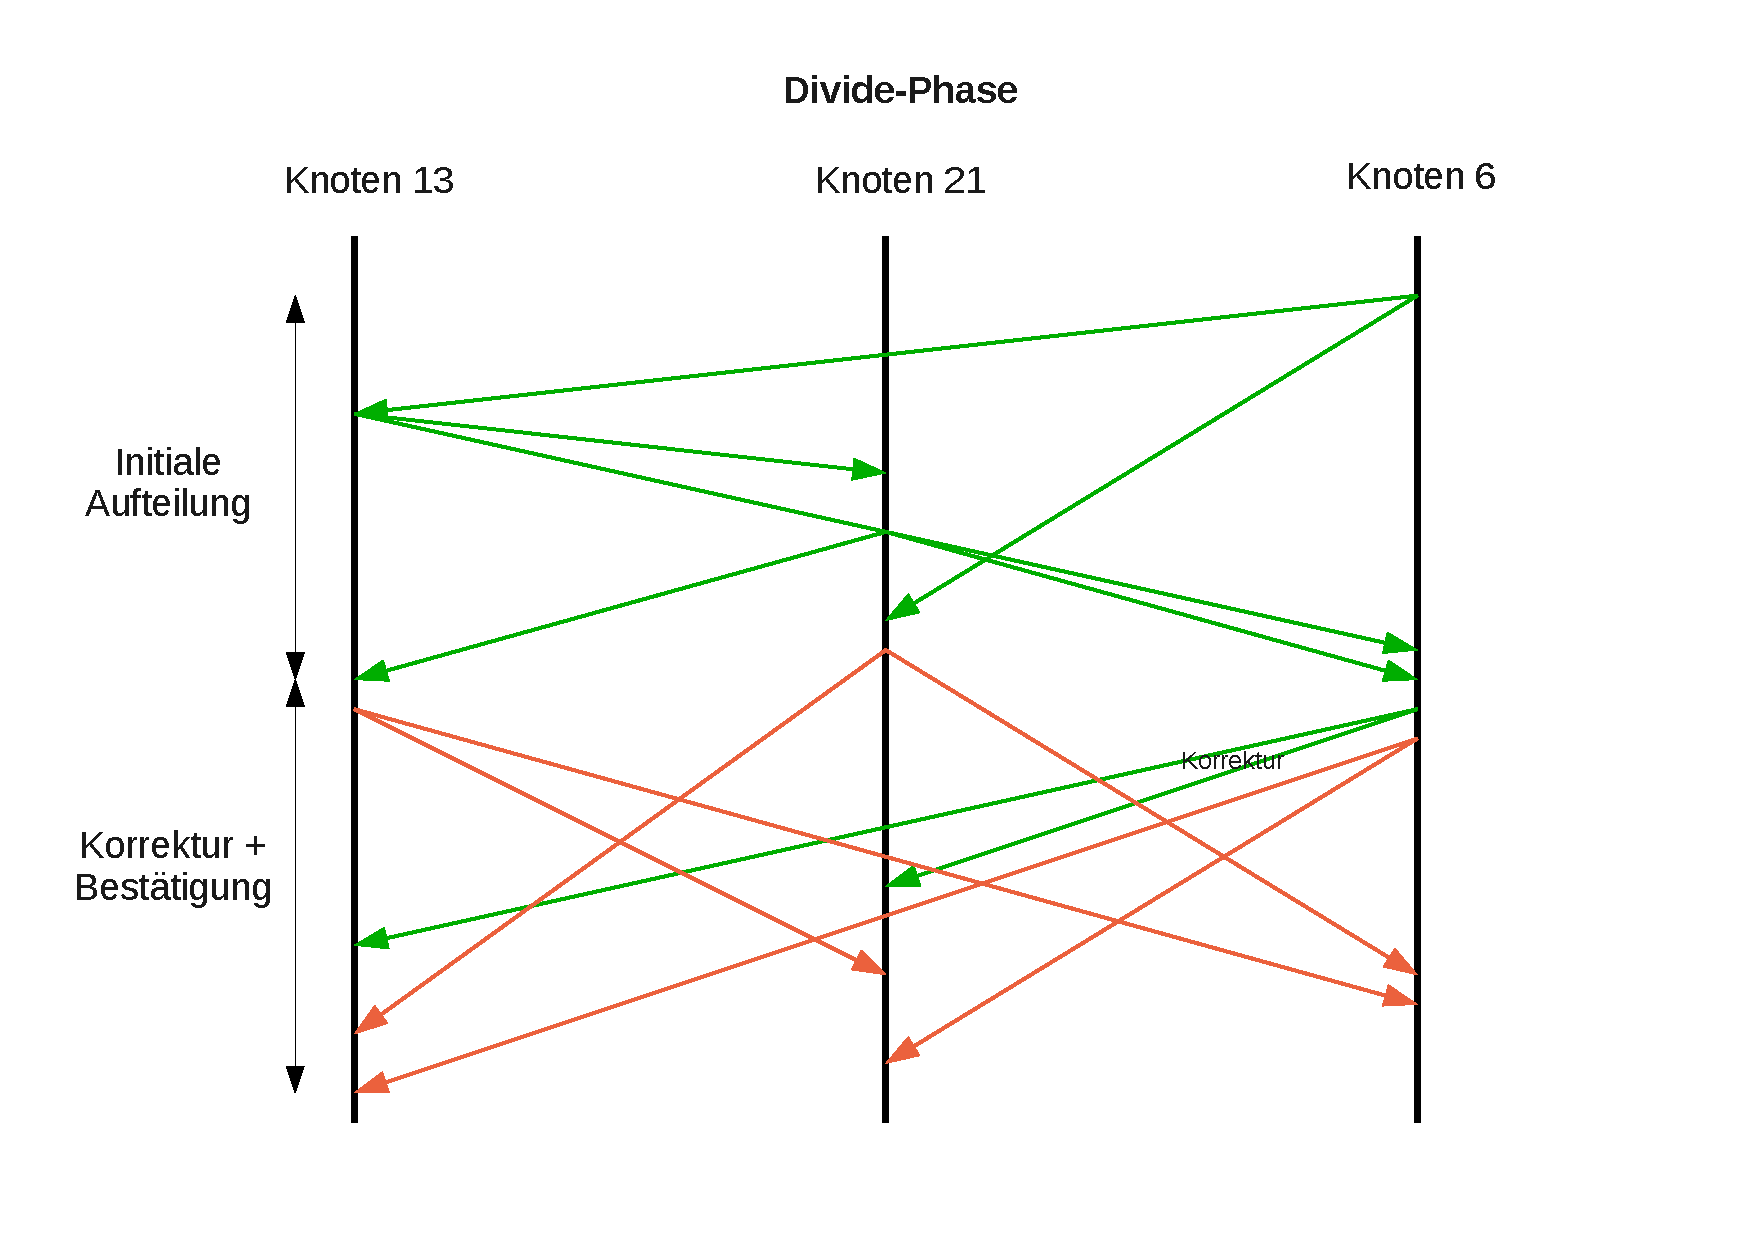
\includegraphics[width=9cm]{../img/recovery_divide}
			\end{block}
		\end{frame}

		\begin{frame}
			\frametitle{FastRecovery}

			\begin{block}{Recover-Phase}
				\center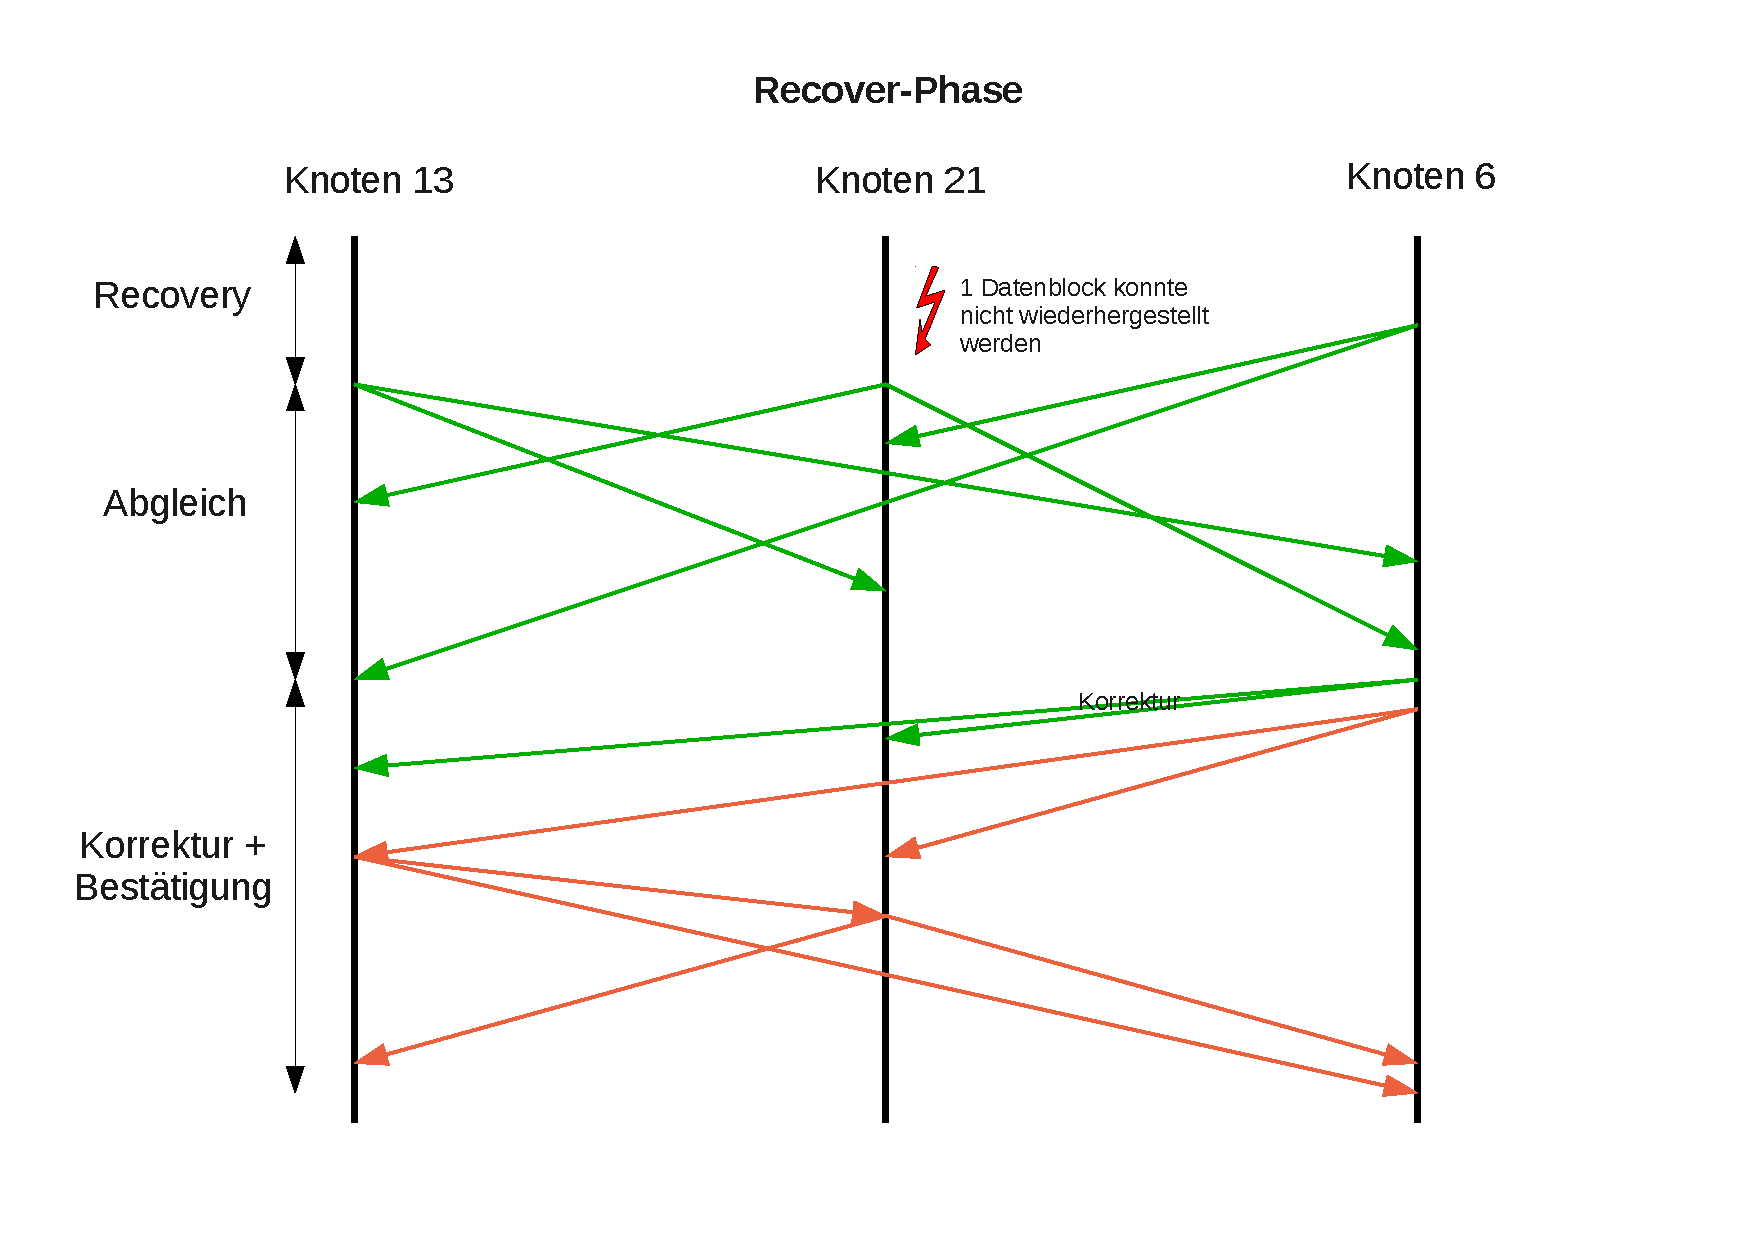
\includegraphics[width=9cm]{../img/recovery_recover}
			\end{block}
		\end{frame}

	\subsection{Netzwerk}

		\begin{frame}
			\frametitle{Netzwerk}

			\begin{block}{Eigenschaften}
				\begin{itemize}
					\item Java NIO
					\item TCP Sockets
					\item drei Nachrichtentypen: Message, Request und Response
					\item automatische Neuübertragung eines Requests nach einem Timeout
					\item Event-Listener-Model:
						\begin{itemize}
							\item \texttt{MessageReceiver} werden über eingehende Nachrichten informiert
							\item \texttt{RequestReceiver} werden über eingehende Requests und Responses informiert
							\item \texttt{ConnectionLostReceiver} werden über unterbrochene Verbindungen informiert
						\end{itemize}
					\item Aufbewahrung von nicht behandelten Nachrichten
				\end{itemize}
			\end{block}					
		\end{frame}

\section*{Danksagung}

		\begin{frame}
			\frametitle{Danksagung}

			\begin{block}{Vielen Dank für Ihre Aufmerksamkeit}
				Für Fragen stehe ich gerne zur Verfügung
			\end{block}
		\end{frame}

\end{document}
